%%%%%%%%%%%%%%%%%%%%%%%%%%%%%%%%%%%%%%%%%
% Thin Sectioned Essay
% LaTeX Template
% Version 1.0 (3/8/13)
%
% This template has been downloaded from:
% http://www.LaTeXTemplates.com
%
% Original Author:
% Nicolas Diaz (nsdiaz@uc.cl) with extensive modifications by:
% Vel (vel@latextemplates.com)
%
% License:
% CC BY-NC-SA 3.0 (http://creativecommons.org/licenses/by-nc-sa/3.0/)
%
%%%%%%%%%%%%%%%%%%%%%%%%%%%%%%%%%%%%%%%%%

%----------------------------------------------------------------------------------------
%   PACKAGES AND OTHER DOCUMENT CONFIGURATIONS
%----------------------------------------------------------------------------------------

\documentclass[11pt]{article} % Font size (can be 10pt, 11pt or 12pt) and paper size (remove a4paper for US letter paper)

\usepackage[utf8]{inputenc} % Set utf8 code
\usepackage[protrusion=true,expansion=true]{microtype} % Better typography
\usepackage[portuguese]{babel}
\usepackage{graphicx} % Required for including pictures
\usepackage{wrapfig} % Allows in-line images
\usepackage[pagebackref]{hyperref}

\usepackage{mathpazo} % Use the Palatino font
\usepackage[T1]{fontenc} % Required for accented characters

\usepackage{wallpaper}
\usepackage[font={color=white,bf},figurename=Fig.,labelfont={it}]{caption}
\usepackage{lipsum, xcolor, etoolbox, footmisc, bigfoot}

\usepackage{tabu}
\hypersetup{
    colorlinks=false,
    pdfborder={0 0 0},
}

\setcounter{secnumdepth}{5}
\setcounter{tocdepth}{5}

\linespread{1.05} % Change line spacing here, Palatino benefits from a slight increase by default

\makeatletter
\renewcommand\@biblabel[1]{\textbf{#1.}} % Change the square brackets for each bibliography item from '[1]' to '1.'
\renewcommand{\@listI}{\itemsep=0pt} % Reduce the space between items in the itemize and enumerate environments and the bibliography

\renewcommand{\maketitle}{ % Customize the title - do not edit title and author name here, see the TITLE block below


\begin{center} % Right align
{\LARGE\@title} % Increase the font size of the title

\vspace{20pt} % Some vertical space between the title and author name

\end{center}
}

\patchcmd{\ps@plain}{\thepage}{\textcolor{white}{\thepage}}{}{}
\makeatother

\begin{document}

\ThisTileWallPaper{\paperwidth}{\paperheight}{res/wallpaper_header.jpg}
\color{white}
\pagestyle{plain}
\def\footnotelayout{\color{white}}
\renewcommand\thefootnote{\textcolor{white}{\arabic{footnote}}}
\begin{titlepage}
 \vfill
  \begin{center}
   {\textbf{{{\Huge  Strife Of Mythology Tower Defense}}}}\\[6cm]


   {{\huge Game Design Document}}\\[6cm]

   \hspace{.45\textwidth} %posiciona a minipage
  \vfill

\vspace{2cm}

\large \textbf{Brasília}

\large \textbf{Abril de 2016}
\end{center}
\end{titlepage}
\newpage
\color{black}
\tableofcontents

\newpage

%----------------------------------------------------------------------------------------
%   DOC BODY
%----------------------------------------------------------------------------------------

\TileWallPaper{\paperwidth}{\paperheight}{res/wallpaper_body.jpg}
\color{white}

\section*{Tabela de Revisão}


\begin{table}[h]

  \taburulecolor{white}
  \color{white}
\begin{tabu}{|l|l|p{60mm}|l|}

\hline 
\textbf{Versão}     & \textbf{Data}     & \textbf{Descrição}                              			& \textbf{Autor}    \\ \hline
0.1                 & 05/03/16        & Objetivo / História / Controles                    			& Marcelo Martins     \\ \hline
0.2                 & 06/03/16        & Requisitos Tecnológicos                            			& Marcelo Martins     \\ \hline
0.3                 & 13/03/16        & Aplicando correções propostas                      			& Marcelo Martins     \\ \hline
0.4                 & 12/04/16      & Adição dos Personagens / Refinamento dos itens anteriores   	& Marcelo Martins     \\ \hline
0.5                 & 29/04/2015        & Rascunho das telas				                   			& Jônntas Lennon     \\ \hline
0.6                 & 10/05/2015        & telas / Personagens				                   			& Jônntas Lennon     \\ \hline
0.7                 & 18/05/2015        & Economia				                   			& Jônntas e Marcelo     \\ \hline
0.8                 & 18/05/2015        & Personagens				                   			& Jônntas e Marcelo     \\ \hline


\end{tabu}
\end{table}

\newpage

\section{Objetivo do jogo}

O \textit{\textbf{SoMTD}} é um jogo de estilo\textit{ Tower Defense}, onde o objetivo é impedir que as \textit{waves} de monstros avancem pela caminho utilizando torres que atacam estas \textit{waves}, estas torres são pertencentes a três Deuses.

 A medida em que as \textit{waves} são vencidas, elas ficam mais fortes e difíceis de derrotar. Nisto haverá um recurso que servirá para evoluir, desbloquear e construir novas torres, o qual será obtido conforme os monstros forem derrotados.

\section{Glossário}
\begin{itemize}
\item Wave: Inimigos que nascem em conjunto em momentos do jogo.
\item Trilha: Caminho pré-determinado que será seguido pelas \textit{waves}. Caso um inimigo chegue ao fim da trilha, o jogador sofre uma punição.
\item Tower Defense: Um estilo de jogo onde um jogador deve impedir unidades inimigas de completarem seu objetivo utilizando torres.
\item HP - Health Point : Atributo referente a vida \textit{player}.
\item Sp - Speed : refere-se a velocidade com que as \textit{waves} se movem.
\item GoldA - Gold reaward  : refere-se a quantia de \textit{gold} ganha ao derrotar o monstro.
\item DiscountHP - Discount Health Point : refere-se a quantia de \textit{HP} perdida quando o monstro atravessar a trilha.
\item Attack Speed - velocidade em segundos que um tiro demora para alcançar uma torre
\item Damage - dano causado pelo ataque de uma torre.
\item Gold: única remuneração do jogo.
\end{itemize} 
 
\section{Conceito do jogo}

As torres pertencem  três Deuses sendo eles:
\begin{itemize}
\item Hades.
\item Zeus.
\item Poseidon.
\end{itemize}

Cada Deus terá um conjunto de quatro Torres a seu dispor, divididas em 4 categorias sendo que cada categoria possuirá uma singularidade em relação as demais, possuindo assim vantagens em relação a alguns tipos de monstros e desvantagens em relação a outros tipos de monstros.

Ao iniciar o jogo, o jogador terá uma quantidade de ouro suficiente para adquirir e colocar torres de forma estratégica, tentando evitar a passagem dos inimigos pela trilha, sendo que no início do jogo apenas um tipo de torre por Deus estará disponível, tais torres podem ser evoluídas ao passo que o jogador consiga evoluir de era. 

A mudança de cenário ocorrerá ao decorrer do jogo, a medida em que as \textit{waves} forem derrotadas o jogador alcançará pontos de performance, que ao completar a barra referente a estes pontos, ocorrerá uma troca de era, havendo assim a mudança de fase e consequentemente de cenário. 

O final do jogo pode-se dar de duas formas:

\begin{enumerate}
\item O jogador posicionou as torres da forma que ele acreditava ser a forma mais estratégica, contudo não era a melhor forma, e ele não conseguiu suportar a \textit{wave},fazendo com que os inimigos cheguem ao final da trilha, com isso ele irá acumular penalidades, atingindo o máximo de penalidades aparecera a mensagem de \textit{Game Over};
\item O jogador consegue posicionar as torres da forma mais estratégica, conseguindo assim, suportar todas as \textit{waves} impostas, caso isso ocorra, ele irá receber uma mensagem de \textit{You Win}.

\end{enumerate}

\section{Gameplay}

\subsection{Progressão do Jogo}

\subsection{Timer}

\newpage

\section{Mecânicas do Jogo}
\subsubsection{Movimentação}
A movimentação das \textit{waves} será em um caminho pré-determinado, cabendo ao jogador apenas posicionar as torres com o mouse próxima a esse caminho, não havendo assim movimentação por parte do jogador principal, caso não seja possível a inserção da torre no local desejado, como a trilha das \textit{waves}, ou um \textit{tiler} já ocupado por outra torre, tem-se um indicativo da impossibilidade de inserção da torre no local.

\subsubsection{Resolução}
A resolução do jogo será de 1124x700 \textit{pixels}, esta resolução deve dar um tamanho confortável para o jogador que terá a disposição um mapa relativamente grande.

Os monstros terão uma resolução que pode variar bastante dependo do artista que desenvolver o protótipo para tal monstro, sendo aconselhável que tenha aproximadamente 30 \textit{pixels} de largura e 50 \textit{pixels} de altura, porém este valor é relativo uma vez que os monstros possuem características físicas diferentes.

Para as torres definimos algo entre 80 a 100 \textit{pixels} de altura e 50 a 70 \textit{pixels} de largura, porém se o artista achar necessário fugir um pouco deste \textit{range}, para melhorar a caracterização do personagem e permanecendo dentro do \textit{Tile}, poderá haver esta mudança.

\subsection{Checkpoints}
O jogo será direto, não havendo \textit{checkpoints} ou seja uma vez morto o jogador terá que reiniciar no inicio da fase, e ao sair do jogo perde-se todo o progresso salvo, porém caso o mesmo avance de fase, os níveis abertos estarão disponíveis para o jogo.

\subsection{Mecânica das Torres}

As torres terão \textit{range} que é um campo de ataque, no qual somente será possível causar dano no monstro caso este esteja no campo de ação da torre.

Como dito na secção Inimigos, quando um inimigo entrar no \textit{range} das torres, as mesmas começarão a atacar os monstros obedecendo a ordem de entradas destes monstros, ou seja a torre continuara atacando o monstro até que este saia do \textit{range} de ataque ou até que o monstro esteja morto, assim atacando um novo monstro somente após estas duas condições.

\begin{figure}[!htp]
\centering
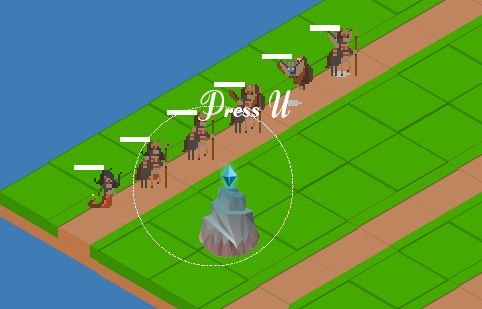
\includegraphics[scale=0.35]{res/atac.png} \quad
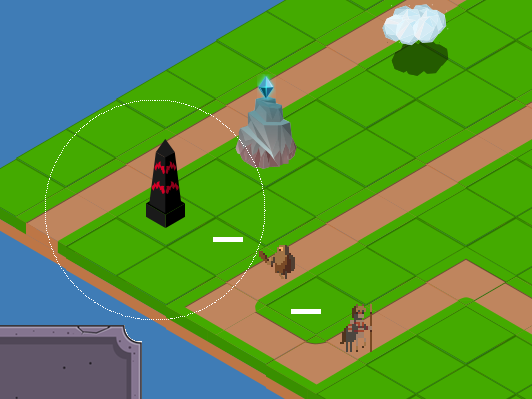
\includegraphics[scale=0.3]{res/dont.png}
\caption{Range de Ataque das torres, na primeira a torre ataca somente o primeiro a entrar no range, na segunda imagem a torre não ataca já que o inimigo encontra-se fora do range}
\label{Tela Barracks}
\end{figure}

\newpage

\section{Câmera e HUD}

\subsection{Câmera}

A câmera do jogo será 2D estática em um mapa isométrico, como exemplificado pela imagem abaixo.
\begin{figure}[!htp]
\centering
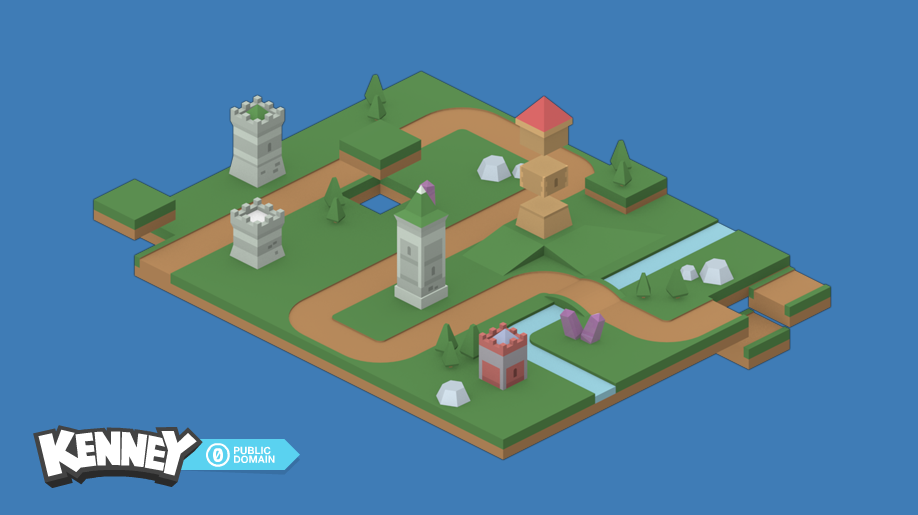
\includegraphics[scale=0.25]{res/map_example.png}
\caption{Tela Câmera}
\label{Tela Barracks}
\end{figure}

\subsection{HUD}

O HUD (Heads-Up Display) será composto de um menu inferior o qual será dividido em três secções, sendo elas:
\begin{itemize}
\item Um box contendo os três Deuses e os botões referentes as eras, ao clicar no Deus ocorre a atualização do menu central que contem as quatros torres deste deus, estas torres terão níveis de poder diferentes iniciando obviamente na mais fraca até a mais forte, ao passar o mouse em cima das torres uma box exibindo as informações referentes a esta torres é exibida.

\begin{figure}[!htp]
\centering
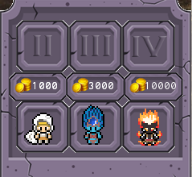
\includegraphics[scale=1]{res/box_dos_deuses.png}
\caption{Box dos Deuses, com os botões das eras e dos deuses}
\label{HUD}
\end{figure}

\item No centro como dito anteriormente tem-se as três torres existentes sendo que as torres disponíveis possuem uma estrela para indicar que as mesmas são selecionáveis, caso a torre esteja bloqueada, um \textit{\textbf{"X"}} ocupa o lugar da estrela. Há também neste box, abaixo da figura das torres uma representação em \textit{gold} alcançada pelas torres deste tipo.
\item No box do conto inferior direito tem-se a torre selecionada, esta torre fica com um tom mais claro no menu central.
\item No canto superior esquerdo tem-se a barra de \textit{HP}, do jogador.
\item Finalizando tem-se no canto superior direito, as informações referentes ao \textit{gold} total alcançado.
\end{itemize}

\begin{figure}[!htp]
\centering
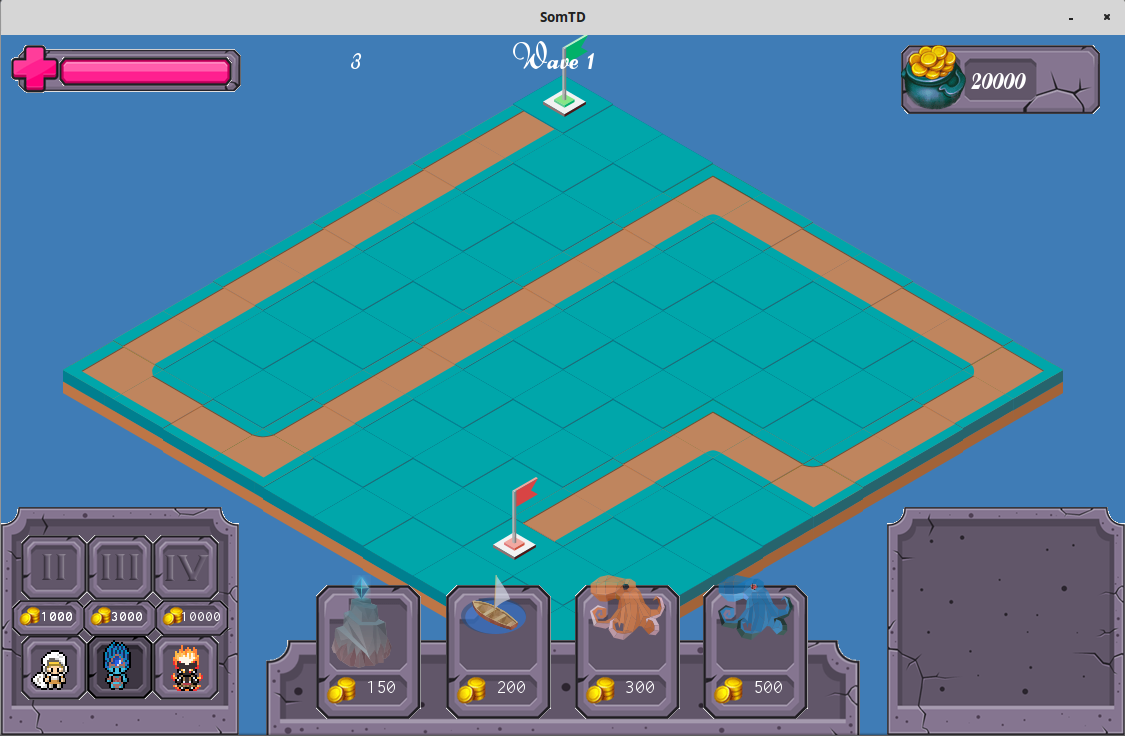
\includegraphics[scale=0.4]{res/gameplay2.png}
\caption{Hud}
\label{HUD}
\end{figure}

\newpage

\section{Personagens Principais}

\subsection{Deuses}
Como dito nas secções anteriores, haverão 3 Deuses:

{\large \textbf{Zeus}}: Zeus é um Deus imortal considerado como o pai dos Desuse e dos homens, tido como o mais poderoso dentre os Desuses do \textit{Olimpo}. É quem exerce a ordem e domínio sobre os outros Deuses, é o Deus dos \textbf{Céus, Raios e Relâmpagos}, tem como conjunge a deusa \textit{Hera}, a deusa da maternidade. 

Diante da ameaça de invasão pelas \textit{waves} de monstros na terra, \textit{Zeus liderará} a tropa de Deuses responsáveis pela derrota destes monstros e vitoria da humanidade. 

Deste modo, sendo um Deus cujo as torres utilizam predominantemente raios para atacar, possuirá dano maior em inimigos do tipo fly.
\begin{figure}[!htp]
\centering
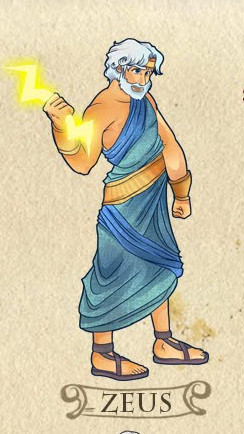
\includegraphics[scale=0.25]{res/characters/zeus.png}
\caption{Imagem conceitual de Zeus}
\label{zeus}
\end{figure}

Zeus é possui a aparência de um senhor sábio, extremamente poderoso e respeitável.

Para a caracterização do personagem foi adotada a técnica de \textit{Pixel-Arte}, uma vez que a equipe de artistas já possuem experiência neste tipo de técnica, otimizando  assim o tempo necessário para o desenvolvimento dos mesmos. Abaixo segue a imagem do personagem com a arte finalizada.

\begin{figure}[!htp]
\centering

\includegraphics[scale=2]{res/characters/zeus_panel.png}
\caption{Pixel-Arte de Zeus}
\label{zeus}
\end{figure}

\newpage

{\large \textbf{Poseidon}}: Poseidon é o Deus supremo do mar, também conhecido como Deus dos terremotos, é um dos irmãos de \textbf{Zeus}, podendo ser tão forte quanto o próprio irmão, mas devido ao fato do irmão \textbf{Zeus} te-lo salvo da barriga de seus pai o Titan \textbf{Chronos}, Poseidon e Zeus selarão um acordo, no qual \textbf{Zeus} seria o Deus supremo do \textbf{Olimpo} e \textbf{Poseidon} manteria o poder absoluto sobre os mares e oceanos. Comandado por Zeus Poseidon utilizara seus poderes para destruir os monstros invasores e restaurar o equilíbrio entre os mundos.

Como suas torres utilizam o poder das águas para atacar, possuirá assim dano maior em  inimigos do tipo \textit{speed}.

\begin{figure}[!htp]
\centering
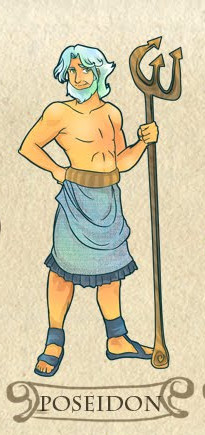
\includegraphics[scale=0.25]{res/characters/poseidom.png}
\caption{Exemplo conceitual de poseidom}
\label{poseidom}
\end{figure}

Para a caracterização deste personagens utilizou-se uma arte predominantemente azul, para simbolizar as águas.

\begin{figure}[!htp]
\centering

\includegraphics[scale=2]{res/characters/poseidon_panel.png}
\caption{Pixel-Arte de Poseidon}
\label{zeus}
\end{figure}

\newpage

{\large \textbf{Hades}}: Hades é o deus dos mortos e do mundo inferior, é o deus mais odiado pelos humanos, não tendo também nenhuma simpatia pelos mesmos, porém ao ser recrutado por \textbf{Zeus}, acaba se juntando ao seu exercito de Deuses e combatendo os monstros invasores.

Sendo um Deus que utiliza maldições para atacar, possuirá dano maior em inimigos do tipo tanker.

\begin{figure}[!htp]
\centering
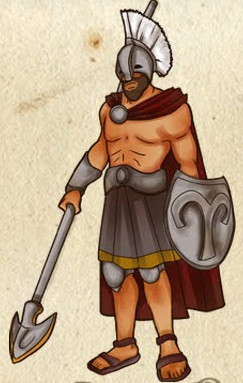
\includegraphics[scale=0.25]{res/characters/hades.png}
\caption{Exemplo conceitual de hades}
\label{satiro}
\end{figure}

Para a caracterização do personagem optou-se por um tom mais sombrio, uma vez que o mesmo é o senhor do mundo dos mortos, assim definiu-se um tom mais escuro e com fogo, representando as chamas do submundo.

\begin{figure}[!htp]
\centering

\includegraphics[scale=2]{res/characters/hades_panel.png}
\caption{Pixel-Arte de Poseidon}
\label{zeus}
\end{figure}

\newpage


\subsection{Torres}
Serão quatro torres para cada Deus, sendo divididas em três níveis, para subir de nível e liberar a torre de \textit{tier} superior é necessário conseguir uma quantia de\textit{gold}, e clicar no botão para a troca de era, estes botões estão posicionados acima dos deuses. A progressão de níveis entre as torres esta descrito na Progresso do jogo e na secção economia, que detalha o valor de cada uma das torres bem como os valores para evoluir as mesmas.

Botão de heras com os respectivos valores para a evolução das eras.
\begin{figure}[!htp]
\centering
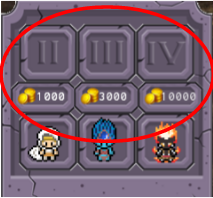
\includegraphics[scale=1]{res/era_button.png}
\caption{Botões de evolução de era}
\label{Butões de evolução de era}
\end{figure}

\paragraph{{\Large Zeus}: As torres associadas à Zeus, terão como ataque raios. Sendo que os ataques, possuem um alto poder, porém demoram um pouco para serem lançados.}

\begin{figure}[!htp]
\centering

\includegraphics[scale=1]{res/projectiles/projetil_zeus2.png}
\caption{Projetil utilizados pelas torres de Zeus.}
\end{figure}

Torre de Zeus 0: Esta torre tem como forma uma nuvem e ataca com raios
\begin{enumerate}
\item Attack Speed 2 segundos.
\item DAmage 50 hp.
\end{enumerate}

\begin{figure}[!htp]
\centering
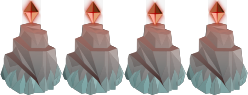
\includegraphics[scale=1]{res/towers/tower_0.png}
\caption{torre de Zeus 0}
\end{figure}

Torre de Zeus 1: Esta torre tem como forma um tufão, sendo mais rápida que a torre 0, e causando o dobro de dano ao monstro.
\begin{enumerate}
\item Attack Speed 1.5 segundos.
\item DAmage 100 hp.
\end{enumerate}

\begin{figure}[!htp]
\centering

\includegraphics[scale=1.3]{res/towers/tower_1.png}
\caption{torre de Zeus 1}
\end{figure}

Torre de Zeus 2: Esta torre tem como forma uma montanha com um raio em cima da mesma, ela ataca com um raio forte e rápido.
\begin{enumerate}
\item Attack Speed 1.5 segundos.
\item DAmage 150 hp.
\end{enumerate}

\begin{figure}[!htp]
\centering
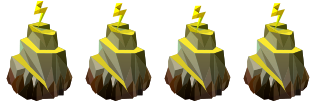
\includegraphics[scale=1.3]{res/towers/tower_2.png}
\caption{torre de Zeus2 }
\end{figure}

Torre de Zeus 3: Esta torre tem como forma uma montanha rodeada com nuvens, por ser a torre de Tier mais elevado, esta possui um ataque bem poderoso em um curto espaço de tempo.
\begin{enumerate}
\item Attack Speed 1 segundos.
\item DAmage 200 hp.
\end{enumerate}

\begin{figure}[!htp]
\centering

\includegraphics[scale=1.3]{res/towers/tower_3.png}
\caption{torre de Zeus 3}
\end{figure}

\newpage

\paragraph{{\Large Poseidon}: As torres associadas à Poseidon, atacarão com ondas de água. Estas torres possuem o menor dano no ataque entre as torres, porém elas ao atacarem colocam os inimigos em velocidade \textit{slow} possuem um poder mediando e uma frequência rápida.}

\begin{figure}[!htp]
\centering

\includegraphics[scale=1]{res/projectiles/projetil_poseidon.png}
\caption{Projetil utilizados pelas torres de Poseidon.}
\end{figure}

Torre Poseidon 16: Esta torre tem como forma uma montanha com um cristal azul em cima da mesma, utiliza como ataque um \textit{slow} em um inimigo próximo. Como é uma torre de \textit{slow} não possui dano.
\begin{enumerate}
\item Attack Speed 3 segundos.
\item DAmage 0 hp.
\end{enumerate}

\begin{figure}[!htp]
\centering

\includegraphics[scale=1]{res/towers/tower_16.png}
\caption{torre Poseidon16}
\end{figure}

Torre Poseidon 17: Esta torre tem como forma um barquinho, é menos lenta que a anterior.
\begin{enumerate}
\item Attack Speed 2 segundos.
\item DAmage 0 hp.
\end{enumerate}

\begin{figure}[!htp]
\centering

\includegraphics[scale=1.3]{res/towers/tower_17.png}
\caption{torre de Poseidon17}
\end{figure}

Torre Poseidon 18: Esta torre tem como forma um Polvo amarelo sendo bem rápida no ataque.
\begin{enumerate}
\item Attack Speed 2 segundos.
\item DAmage 0 hp.
\end{enumerate}

\begin{figure}[!htp]
\centering

\includegraphics[scale=1.3]{res/towers/tower_18.png}
\caption{torre de Poseidon18}
\end{figure}

Torre Poseidon 19: Esta torre tem como forma um Polvo Azul, por ser extremamente rápida, consegue atingir inúmeros monstros..
\begin{enumerate}
\item Attack Speed 2 segundos.
\item DAmage 0 hp.
\end{enumerate}

\begin{figure}[!htp]
\centering

\includegraphics[scale=1.3]{res/towers/tower_19.png}
\caption{Poseidon19}
\end{figure}

\newpage

\paragraph{{\Large Hades}: As torres associadas à Hades, atacarão com bolas de fogo. Sendo que os ataques, possuem um poder mediando e uma frequência rápida.}

\begin{figure}[!htp]
\centering

\includegraphics[scale=1]{res/projectiles/projetil_caveira.png}
\caption{Projetil utilizados pelas torres de Hades.}
\end{figure}

Torre Hade 32: Esta torre tem como forma um Obelisco, tem um ataque bem rápido funcionando quase como uma metralhadora, assim mesmo que seus tiros sejam relativamente fracos é uma torre forte.
\begin{enumerate}
\item Attack Speed 03 segundos.
\item Damage 20 hp.
\end{enumerate}

\begin{figure}[!htp]
\centering
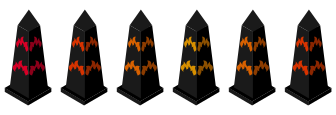
\includegraphics[scale=1]{res/towers/tower_32.png}
\caption{torre Hades32}
\end{figure}

Torre Hade 33: Esta torre tem como forma uma caveira roxa, possui um ataque de \textit{poison} que troca a cor do inimigo para verde.
\begin{enumerate}
\item Attack Speed 0.3 segundos.
\item DAmage 30 hp.
\end{enumerate}

\begin{figure}[!htp]
\centering
\advance\leftskip-3cm
\advance\rightskip-3cm

\includegraphics[scale=1.3]{res/towers/tower_33.png}
\caption{torre de Hades33}
\end{figure}

Torre Hade 34: Esta torre tem como forma uma caveira verde, possui um ataque de rápido.
\begin{enumerate}
\item Attack Speed 0.2 segundos.
\item DAmage 30 hp.
\end{enumerate}

\begin{figure}[!htp]
\centering
\advance\leftskip-3cm
\advance\rightskip-3cm

\includegraphics[scale=1.3]{res/towers/tower_34.png}
\caption{torre de Hades34}
\end{figure}


Torre Hade 35: Esta torre tem como forma uma caveira em cima de um mastro, é a torre mais rápida.
\begin{enumerate}
\item Attack Speed 0.1 segundos.
\item DAmage 30 hp.
\end{enumerate}

\begin{figure}[!htp]
\centering

\includegraphics[scale=1.3]{res/towers/tower_35.png}
\caption{Hades35}
\end{figure}


\section{Inimigos}
\subsection{Waves} 

Haverão diversas \textit{waves}, onde os monstros estarão divididas entre 4 categorias, sendo elas normal, tanker, fly e  speed, a principio não haverá um monstro \textit{Boss}, caso o jogo evolua poderia-se pensar em um \textit{boss}.

As \textit{waves} sempre nascerão no mesmo lugar, que pode ser alternado somente entre as fases do jogo, este lugar é indicado com uma bandeira verde, ao nascer as \textit{waves} farão sempre o mesmo caminho seguindo a trilha pre-definida e indicada por uma cor diferente no mapa com o final da trilha indicado com uma bandeira vermelha, mantendo uma velocidade constante da sua categoria de \textit{waves}. 

As \textit{waves} não interagirão no cenário ou seja não atacarão as torres nem possuirão um mecanismo para evitar ataques das torres, ou seja ao entrar no campo de visão de ataque de uma torre as \textit{waves} serão atacadas, porém caso a torre já esteja atacando um monstro esta continuara atacando a este monstro enquanto o monstro tiver no campo de visão da torre.

Para a derrota da \textit{wave}, serão atribuídos \textit{golds} para cada monstro derrotado. 

Cada monstro terá uma quantia de \textit{HP} especifica variando de acordo a sua categoria, no qual eles somente serão derrotados ao zerar este \textit{HP}, e caso isto ocorrer eles automaticamente somem do mapa e uma quantia de \textit{gold} é atribuída ao jogador.

As \textit{waves} terão uma quantia de inimigos randômica, podendo variar entre as fases, e os monstros serão inseridos randomicamente nas \textit{waves}.

Devido ao tempo de desenvolvimento de jogo não haverá diferenciação de inimigos por fases no jogo, isto acarretaria um esforço gigantesco na criação de personagens uma vez que por fase são 4 categorias diferentes de inimigos, ocasionando um grande trabalho inicialmente desnecessário. 

\subsection{categorias}
Descrição dos inimigos pertencentes as \textit{waves}:

Os inimigos serão inseridos randomicamente nas fases do jogo, no caso serão desenvolvidas somente três níveis, que alternam somente o mapa e cenário do jogo, não havendo diferenciação dos inimigos nos níveis que compõem o jogo.

Tem-se para todos os inimigos quatro tipos de cores, a normal e outras três verde, azul e vermelho, que são ativadas no ataque de torres especificas. 

\textbf{{\large Normal}} – na primeira categoria de inimigos tem-se os inimigos do tipo normal, estes não terão nenhum beneficio sendo bem equilibrados e aparecerão em maior quantidade. Esta categoria de monstro será representada pelo \textit{ciclope}.
\begin{itemize}
\item HP - 100
\item Sp - 200 milesegundos.
\item DiscountHP - 1 \textit{hp's}.
\item GoldR - 10 golds.
\end{itemize}

\begin{figure*}[!htp]
\centering
\advance\leftskip-3cm
\advance\rightskip-3cm

\includegraphics[scale=2]{res/units/ciclope/cyclop.png} \quad

\includegraphics[scale=1]{res/units/ciclope/ciclopsheet.png} \quad

\includegraphics[scale=1]{res/units/ciclope/ciclopsheet_congelado.png} \quad

\includegraphics[scale=1]{res/units/ciclope/ciclopsheet_verde.png} \quad

\includegraphics[scale=1]{res/units/ciclope/ciclopsheet_vermelho.png} 
\caption{Spritsheet esquerda-direita do ciclope.}
\label{ciclopesheet}
\end{figure*}

\newpage
\textbf{{ {\large Speed}}} – A\textbf{Meduza} representa o tipo \textit{speed}, sendo bem rápida, porém com um baixo \textit{hp}, e será como dito na mitologia grega uma mulher com cabeça de cobra e neste casso com um corpo de cobra abaixo da cintura.

\begin{itemize}
\item HP - 80
\item Sp - 80 milesegundos.
\item DiscountHP - 2 \textit{hp's}.
\item GoldR - 15 golds.
\end{itemize}

\begin{figure}[!htp]
\centering

\includegraphics[scale=4]{res/characters/medusa.png}
\caption{Meduza do jogo}
\label{Medusa}
\end{figure}

\begin{figure*}[!htp]
\centering
\advance\leftskip-3cm
\advance\rightskip-3cm

\includegraphics[scale=]{res/units/medusa/medusasheet.png} \quad

\includegraphics[scale=1]{res/units/medusa/medusasheet_congelada.png} \quad

\includegraphics[scale=1]{res/units/medusa/medusasheet_verde.png} \quad

\includegraphics[scale=1]{res/units/medusa/medusasheet_vermelho.png} 
\caption{Spritsheet esquerda-direita do ciclope.}
\label{ciclopesheet}
\end{figure*}

\newpage

\textbf{{\large Tanker}} – Os \textit{Centauros}, serão os inimigos do tipo \textit{Tanker}, possuindo um alto \textit{hp} e uma alta recompensa em \textit{golds}, porém uma mobilidade reduzida possuirão, além disso estes inimigos retiram uma alta quantia de \textit{hp}.

\begin{itemize}
\item HP - 400
\item Sp - 250 milesegundos.
\item DiscountHP - 4 \textit{hp's}.
\item GoldR - 40 golds.
\end{itemize}

\begin{figure}[!htp]
\centering
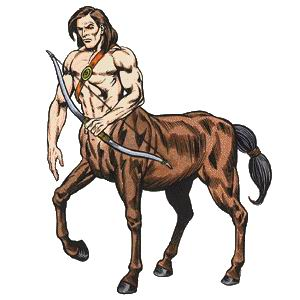
\includegraphics[scale=0.4]{res/characters/centauro.jpg} \quad

\includegraphics[scale=3]{res/characters/centauro.png} 
\caption{Exemplo de centauros e pixel-art do centauro}
\label{cyclops}
\end{figure}

\begin{figure*}[!htp]
\centering
\advance\leftskip-3cm
\advance\rightskip-3cm

\includegraphics[scale=2]{res/units/centauro/centauro.png} \quad

\includegraphics[scale=0.7]{res/units/centauro/centaurosheet.png} \quad

\includegraphics[scale=0.7]{res/units/centauro/centaurosheet_congelado.png} \quad

\includegraphics[scale=0.7]{res/units/centauro/centaurosheet_verde.png} \quad

\includegraphics[scale=0.7]{res/units/centauro/centaurosheet_vermelho.png} 
\caption{Spritsheet esquerda-direita do centauro.}
\label{centaurosheet}
\end{figure*}

\newpage

\textbf{{\large Fly}} – As \textit{Harpias} são os inimigos do tipo\textit{Fly}, serão inimigos rápidos, porém com hp um pouco acima do normal, que possuirão uma fraca recompensa em gold, porém terão um alto impacto no \textit{hp}.

\begin{itemize}
\item HP - 80
\item Sp - 80 milesegundos.
\item DiscountHP - 2 \textit{hp's}.
\item GoldR - 15 golds.
\end{itemize}

\begin{figure}[!htp]
\centering
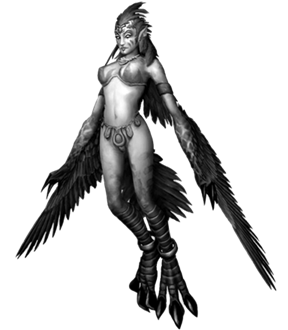
\includegraphics[scale=0.75]{res/characters/harpia.png} \quad

\includegraphics[scale=2]{res/characters/bat.png} 
\caption{harpia conceito inicial}
\label{harpia}
\end{figure}

\begin{figure*}[!htp]
\centering
\advance\leftskip-4cm
\advance\rightskip-3cm

\includegraphics[scale=2]{res/units/harpia/preharpia.png} \quad

\includegraphics[scale=0.7]{res/units/harpia/harpiasheet.png} \quad

\includegraphics[scale=0.7]{res/units/harpia/harpiasheet_congelado.png} \quad

\includegraphics[scale=0.7]{res/units/harpia/harpiasheet_verde.png} \quad
\includegraphics[scale=0.7]{res/units/harpia/harpiasheet_vermelho.png} 
\caption{Spritsheet esquerda-direita da harpia.}
\label{harpiasheet}
\end{figure*}

\newpage

\section{Gameplay do jogo}
\subsection{Níveis}

\begin{enumerate}
\item Título do nível.
	\begin{enumerate}
	\item Mapa 1 - Poseidon
		\begin{enumerate}
		\item \textbf{Breve descrição do nível}: Este mapa tem como inspiração o mar, terreno do todo poderoso rei dos mares Poseidon, além de ter um mapa um pouco mais fácil que os demais, isto com o intuito de ambientar o jogador com os botões e a mecânica do jogo em se, portanto este mapa tem um inicio relativamente fácil, mas evolui rapidamente a um nível de dificuldade aceitável.
		\item \textbf{objetivo do jogador ao longo do nível:} Assim como em todos os níveis, este tem como objetivo resistir as \textit{waves}, matando todos os monstros que surgirem. Porém este nível como dito anteriormente tem como objetivo secundário ambientar o jogador ao jogo.
		\item \textbf{Mecânicas do nível:} Posicionar as torres no podendo evolui-las ao longo da partida.
		\item \textbf{Inimigos encontrados:} Como não há variação de inimigos ao longo dos níveis este e todos os níveis do jogo terão quatro inimigos, descritos na secção inimigos, sendo eles: Ciclope, Harpia, Centauro e Medusa.
		\item \textbf{Visual :} Este nível por ser inspirado no Poseidon, possui um mapa com tiles azuis e um fundo de uma imagem grega de domínio publico bastante inspirada na mitologia grega, sendo ela:
		
			\begin{figure}[!htp]
			\centering
			\includegraphics[scale=0.3]{res/nivel1.png}
			\caption{Nivel 1}
			\label{nivel1}
			\end{figure}
			
			\textbf{Titulo}: La Barca de Caronte/The Boat of Charon (1919).
			\textbf{Autor}: Jose Benlliure y Gil
			\textbf{Ano}: 1855-1937
			\textbf{Copyright}: Public Domain 
			
		\item \textbf{Músicas e efeito sonoros:}
			\textbf{Com relação aos efeitos sonoros, não ha diferenciação entre os níveis, sendo que uma lista e a descrição dos mesmos pode ser encontrado na secção \textit{efeitos sonoros}}.
			\textbf{Música:} a musica deste nível é bem sinfônica, com um tom de sum suspense relativo.
		\end{enumerate}
	\item Mapa 2 - Zeus
		\begin{enumerate}
		\item \textbf{Breve descrição do nível}: Este mapa tem como inspiração o olimpo, o terreno do pai dos Deuses Zeus. Este nível possui um nível de dificuldade superior ao anterior, com as \textit{waves} iniciando em um estado com mais monstros que o anterior sendo necessário uma quantidade bem mais elevada de torres para o jogador conseguir exito. 
		\item \textbf{objetivo do jogador ao longo do nível:} Como o nível de dificuldade aumentou, o objetivo deste nível para derrotar as \textit{waves} é conseguir fazer uma boa combinação dos poderes das torres. 
		\item \textbf{Mecânicas do nível:} Posicionar as corretamente as torres.
		\item \textbf{Inimigos encontrados:} Como dito anteriormente não há variação de inimigos em relação aos níveis.
		\item \textbf{Visual :} Este nível por ser inspirado no Olimpo, possui um mapa com tiles verdes e um fundo de uma imagem grega de domínio publico bastante inspirada em Zeus, sendo ela:
		
			\begin{figure}[!htp]
			\centering
			\includegraphics[scale=0.3]{res/nivel2.png}
			\caption{Nivel 2}
			\label{nivel1}
			\end{figure}
			
			\textbf{Titulo}: The Barque of Charon, Sleep, Night and Morpheus.
			\textbf{Autor}: Giordano, Luca
			\textbf{Ano}: 1684-1686
			\textbf{Copyright}: Public Domain 
		\item \textbf{Músicas e efeito sonoros:}
			Mantem-se os mesmos efeitos sonoros do nível anterior.
			\textbf{Música:} Esta musica é um pouco mais agitada que a anterior, possuindo bastante tambores.
		\end{enumerate}
	\item Mapa 3 - Hades
		\begin{enumerate}
		\item \textbf{Breve descrição do nível}: Este mapa tem como inspiração o submundo dominado por \textit{Hades}, neste nível tem-se a dificuldade máxima implementada no jogo.
		\item \textbf{objetivo do jogador ao longo do nível:} sobreviver o máximo possível e derrotar todas as \textit{waves}.
		\item \textbf{Mecânicas do nível:} Posicionar as corretamente as torres.
		\item \textbf{Inimigos encontrados:} Como dito anteriormente não há variação de inimigos em relação aos níveis.
		\item \textbf{Visual :} Este nível por ser inspirado no submundo, possui um mapa com tiles marrom e um fundo de uma imagem do \textit{caronte}, carregando almas até o submundo 
		
			\begin{figure}[!htp]
			\centering
			\includegraphics[scale=0.3]{res/nivel3.png}
			\caption{Nivel 3}
			\label{nivel3}
			\end{figure}		
			
			\textbf{Titulo}: Charon Carries Souls Across the River Styx.
			\textbf{Autor}: Alexander Litovchenko
			\textbf{Ano}: 1861
			\textbf{Copyright}: Public Domain 
		\item \textbf{Músicas e efeito sonoros:}
			Mantem-se os mesmos efeitos sonoros do nível anterior.
			\textbf{Música:} Como essa fase é mais longa, a musica é um pouco menos estressante.
		\end{enumerate}
	\end{enumerate}	
\item Troca de níveis.
\end{enumerate}
\newpage
		
\begin{figure}[!htp]
\centering
\advance\leftskip-3cm
\advance\rightskip-3cm
\includegraphics[scale=0.75]{res/beatCheart.png}
\caption{Beat Cheart}
\label{nivel3}
\end{figure}		
			

\section{Saúde}

O jogador terá uma barra de vida com 100 HP, esta barra não conterá valores visíveis ao jogador, sendo uma longa barra vermelha no canto superior esquerdo, a qual terá o símbolo em formato de cruz vermelha, mundialmente conhecido como símbolo de saúde.

\begin{figure}[!htp]
\centering
\includegraphics[scale=0.3]{res/saude.png}
\caption{Demonstração da Saúde no mapa do jogo}
\label{Saúde}
\end{figure}
 
A barra de hp decairá a medida que os inimigos atravessem o mapa, sendo que cada tipo de inimigo tem uma pontuação diferente, tal valor esta descrito na secção inimigos, no tópico \textbf{DiscountHP}:

\subsection{Game Over}
O \textit{game Over} só ocorrera se a barra de \textbf{HP} for zerada, assim quando ocorrer uma grande mensagem cobrira a tela do jogo com a frase de \textbf{Game Over}, e as opções para uma nova partida ou para fechar o jogo.

\begin{figure}[!htp]
\centering
\includegraphics[scale=0.3]{res/game_over.png}
\caption{Tela de Game Over}
\label{Game Over}
\end{figure}
\newpage

\section{Economia}

A única remuneração do jogo será em \textit{gold}, o qual terá como intuito incrementar as torres, não havendo nenhum tempo especifico para a compra de torres, exceto o tempo inicial de jogo, que o jogador seleciona as torres desejadas antes do jogo iniciar de fato, assim as compras podem ser realizadas em qualquer momento da partida.

Os \textit{golds}, são acumulativos ao decorrer das fases, sendo perdidos somente no \textit{game over}.

Toda pontuação do jogador será obtido através dos monstros derrotados, quanto mais forte for o inimigo  maior será a recompensa em ouro, sendo que cada um dos monstros possuem uma pontuação diferente, tal pontuação possui os seguinte valores:

\begin{itemize}
 \item Norma = 10 Golds
 \item Tanker = 40 Golds
 \item Speed = 15 Golds
 \item Fly = 8 Golds
 \end{itemize} 
 
Como as torres tem quatro \textit{Tiers}, haverá valores diferentes para as torres de cada \textit{Tiers}, assim para as torres de \textit{Tier 1}, ou seja de nível mais baixo, serão necessários 150 \textit{Golds} para aquisição das mesmas, já para as torres de \textit{Tier 2} será necessária a quantia de 200 \textit{golds} para aquisição das mesmas, caso estas estejam disponíveis.

\begin{itemize}
 \item Tier 1 = 150 Golds
 \item Tier 2 = 200 Golds
 \item Tier 3 = 300 Golds
 \item Tier 4 = 500 Golds
 \end{itemize} 
 
 
Não haverá diferenciação nos valores entre as torres por Tier, ou seja uma torre de tier 1 do Zeus custa o mesmo valor que uma torre de Tier 1 do Poseidon.Assim cada Deus terá torres em todos os \textit{Tiers} existentes.
 
No inicio do jogo, tem-se disponível a quantia de 1000 golds em ouro, suficiente para a compra de alguns torres que pode ser de investidas nas torres de qualquer um dos Deuses.
 
O \textit{gold} será representado por um imagem de ouro e uma quantia ao lado da imagem, essa representação será posicionada no canto superior direito da tela. Também tem-se uma imagem contendo o valor de \textit{gold} alcançado por cada torre existente, este valor fica no HUD abaixo da torre em questão.

\begin{figure}[!htp]
\centering
\includegraphics[scale=1.25]{res/gold.png}
\caption{Representação Gold}
\label{Tela Equip}
\end{figure}

\begin{figure}[!htp]
\centering
\includegraphics[scale=1.0]{res/torresGold.png}
\caption{Representação Gold associado as torres.}
\label{Tela Equip}
\end{figure}

\newpage

\section{Pontuação}
Como descrito na secção Economia, o jogo terá somente um sistema de pontuação, em \textit{golds}, não havendo demais itens de suporte ao jogador.

Devido ao tempo de projeto a equipe decidiu concentrar esforços no desenvolvimento do \textit{gameplay} do jogo, portanto definiu-se que não seria criado um sistema de \textit{Ranking}, assim os golds pertencerão jogador durante a partida, sendo perdidos ao final do jogo, futuramente se for possível, após o final do desenvolvimento do \textit{gameplay} do jogo, no tempo de projeto da disciplina, pode-se criar um sistema local de \textit{Ranking}, porém como dito anteriormente este \textit{Ranking} não é prioridade, caso seja desenvolvido deve ser tratado como um extra ao projeto.  

\begin{figure}[!htp]
\centering
\includegraphics[scale=0.3]{res/pontuacao.png}
\caption{Demontração da pontuação no mapa do jogo}
\label{pontuacao}
\end{figure}
 

\section{Esquema de controle e interface com o usuário}

O jogador movimentará somente o mouse, utilizando o mesmo para colocar as torres na posição desejada, sendo que o mesmo seleciona a torre desejada no menu inferior, o mouse indica que a torre foi selecionada, com a torre sobrepondo o cursor do mouse.

Um circulo em volta do cursor será formado, para indicar o alcance de ataque da torre, caso o local para adicionar a torre sejá inválido este circulo ficará avermelhado.  

\newpage

\section{Front End}

O \textit{Front End} do jogo terá  quatro telas principais, sendo elas, menu de \textit{Abertura}, \textit{Fases}, \textit{Gameplay} e \textit{Créditos}, além de uma tela auxiliar de carregamento \textit{loading screen}. A seguir uma representação das telas do jogo.

\subsection{Tela de Abertura}
A tela de abertura do jogo dará acesso para outras duas telas, que são: \textit{Gameplay} e \textit{Credits}.

Nesta tela haverá a imagem do jogo ao fundo, e um menu com as seguintes opções para o jogador: 
\textit{Play Game} que levará o jogador para a tela de \textit{Gameplay}.
\textit{Crédits} para exibição dos créditos.
\textit{Exit} que fechara o jogo.
Estes botões serão pretos, e quando o jogador passar o mouse por cima destes botões, eles ficarão brancos.\\

\begin{figure}[!htp]
\centering
\includegraphics[scale=0.4]{res/menu_display.png}
\caption{Tela de Abertura}
\label{Abertura}
\end{figure}

\newpage

\subsection{Tela de Gameplay}

Tela principal do jogo, nesta tela tem-se um menu na parte inferior da tela, com as informações das torres de cada Deus no quadro inferior direito, ao clicar no Deus abre-se um menu na parte inferior do mapa com as torres associadas a este deus. Ao selecionar uma torre a mesma passa a ocupar o lugar do mouse até ser posicionada.

Para adicionar uma nova torre o jogador deverá clicar no deus, e depois no torre no quadro inferior central e arrasta a torre no mapa até a posição desejado. Há também em cada torre um pequeno quadro indicando quanto de \textit{gold} custa esta torre.

Para a evolução das eras, tem-se três botões no box inferior esquerdo, no qual o jogador ao clica-lo comprido os requisitos e com a quantia de gold necessária evolui de era.

O mapa fica no centro da tela, ocupando o máximo de área possível.

Na parte superior direita haverá uma barra indicando a \textit{hp} do jogador

Na parte superior direita tem-se um box indicando a quantia de gold disponível do jogador.

\begin{figure}[!htp]
\centering
\includegraphics[scale=0.3]{res/gameplay_display.png}
\caption{Tela de Gameplay}
\end{figure}

Na parte superior central tem-se informações sobre as \textit{waves}, tem-se também um relógio, que aparece ante do inicio de uma nova \textit{wave}.

\begin{figure}[!htp]
\centering
\includegraphics[scale=0.3]{res/gameplay2.png}
\caption{Tela de Gameplay, com o time das waves e com a box de torres aberta.}
\end{figure}

\newpage
\subsection{Tela de Créditos}

Na tela de \textit{Cr} exibe-se o nome e a função de cada um dos integrantes da equipe, sendo de \textit{Desenvolvimento}, \textit{artes} e \textit{música}.

\begin{figure}[!htp]
\centering
\includegraphics[scale=0.3]{res/credits_display.png}
\caption{Logo da SDL}
\label{Logo da SDL}
\end{figure}

\newpage

\subsection{Logo}

A logo a seguir o logo do SomTD].
\begin{figure}[!htp]
\centering
\includegraphics[scale=1.1]{res/logo.png}
\caption{Logo do SomTD}
\label{Logo do SomTD}
\end{figure}

A logo a seguinte representa a API utilizada durante o desenvolvimento.

\begin{figure}[!htp]
\centering
\includegraphics[scale=0.3]{res/Sdl-logo.png}
\caption{Logo da SDL}
\label{Logo da SDL}
\end{figure}

\begin{figure}[!htp]
\centering
\includegraphics[scale=0.3]{res/classification.png}
\caption{Classificação Indicativa}
\label{Classificação Indicativa}
\end{figure}

\begin{figure}[!htp]
\centering
\includegraphics[scale=0.3]{res/capa_do_jogo.png}
\caption{Tela de divulgação}
\label{Classificação Indicativa}
\end{figure}

A classificação indicativa definida foi de 12 anos, devido a possíveis traços de violência no jogo, . 


\newpage

\section{Músicas e Efeitos Sonoros}
\subsection{Músicas}
Para a composição da musica do jogo tem-se três categorias uma abertura, fases créditos. 

\begin{enumerate}
\item 
\textbf{Nome:} Musica de Abertura

\textbf{Descrição:} Esta musica será sinfônica e curta ocorrendo em \textit{loop}, inspirada em jogos famosos como \textit{Mario} e principalmente \textit{Zelda}, assim deve ser uma música "exuberante" e chamativa de modo a ser identificada.

\textbf{Utilização:} será utilizada na tela de abertura do jogo.

\item
\textbf{Nome:} Gameplay

\textbf{Descrição:} Esta musica tem como intuito deixar o jogador confortável durante o jogo, assim deve ter uma melodia tranquila uma vez que a mesma será reproduzida em \textit{loop} durante a partida, assim será uma musica semelhante a "musica de elevador", calma com poucos picos, para evitar que a mesma acabe por "competir" com os efeitos sonoros do jogo, mesmo que sejam poucos.  

\textbf{Utilização:} essa musica será utilizada durante todo o \textit{gameplay} do jogo.

\item
\textbf{Nome:} Créditos

\textbf{Descrição:} Musica a ser exibida durante os créditos, esta é uma música de comemoração portanto deve ser uma música alegre e de preferencia eletrônica. 

\textbf{Utilização:} Utilizada na tela de créditos.
\end{enumerate}

\subsection{Efeitos Sonoros}

\begin{LARGE}
\textbf{Waves}
\end{LARGE}

\begin{enumerate}
\item \begin{itemize}
\item \textbf{Nome:} Anuncio de waves.
\item \textbf{Descrição:} Tintilar de sino indicando que uma nova wave esta chegando. 
\item \textbf{Utilização:} com 2 segundos para a entrada de uma nova \textit{wave}.
\end{itemize}
\item \begin{itemize}
\item \textbf{Nome:} Som referente ao tipo.
\item \textbf{Descrição:} barulho característico ao tipo de monstro.
\item \textbf{Utilização:} na entrada do monstro no campo.
\end{itemize}
\item {\LARGE \textbf{Torres}}
\begin{itemize}
\item \textbf{Nome:} Som de ataque.
\item \textbf{Descrição:} como cada Deus terá duas torres, tem-se duas sons de ataque diferentes um para cada torre, porém nestes três tipos de ataque acontecem variações de sons referentes ao deus associado a torre.
\item \textbf{Utilização:} 
\end{itemize}
\item \begin{itemize}
\item \textbf{Zeus}: Ao atacarem as torres terão variações de ataques com ruídos de raios e trovões.
\item \textbf{Hades}: Para as torres de \textit{Hades}, tem-se variações ruídos de magia, semelhantes ao barulho de fumaça dos filmes.
\item \textbf{Poseidon}: Para as torres do Poseidon, tem-se sons semelhantes ao barulho de água batendo no chão além de ondas de água.
\end{itemize}
\item {\LARGE \textbf{Cenário}}

\begin{itemize}
\item \textbf{Nome:} Tilintar de moedas
\item \textbf{Descrição:} um barulho de tilintar de moedas para indicar que houve alteração no \textit{gold} durante a compra de uma torre. 
\item \textbf{Utilização:} é utilizado quando o \textit{gold} do jogador é reduzido.
\end{itemize}
\item \begin{itemize}
\item \textbf{Nome:} Vitoria
\item \textbf{Descrição:} Uma dublagem semelhante a frase "\textit{You wim}" de jogos antigos, com um barulho de fundo semelhante a um "\textit{tam tanram}".
\item \textbf{Utilização:} é utilizada quando o jogador vence as \textit{waves}.
\end{itemize}
\item \begin{itemize}
\item \textbf{Nome:} Derrota
\item \textbf{Descrição:} Semelhante ao efeito de vitoria porém esta é inspirada na derrota de jogos como "God of War" ou "Mortal Kombat", sendo algo parecido com um tintilar de metais, além de uma frase parecida com "\textit{You Lose}".
\item \textbf{Utilização:} utilizada quando o jogador morre.
\end{itemize}
\item \begin{itemize}
\item \textbf{Nome:} Click.
\item \textbf{Descrição:} som de espada.
\item \textbf{Utilização:} utilizado no menu de abertura.
\end{itemize}
\item \begin{itemize}
\item \textbf{Nome:} Hp baixando.
\item \textbf{Descrição:} som indicando que o hp baixou.
\item \textbf{Utilização:} utilizado quando um monstro atravessa a trilha.
\end{itemize}
\item \begin{itemize}
\item \textbf{Nome:} Level up.
\item \textbf{Descrição:} som indicando a troca de eras.
\item \textbf{Utilização:} na troca de eras.
\end{itemize}
\item \begin{itemize}
\item \textbf{Nome:} Local invalido
\item \textbf{Descrição:} som indicando que o jogador tentou colocar uma torre em um local invalido.
\item \textbf{Utilização:} ao tentar posicionar uma torre em um local invalido.
\end{itemize}
\item \begin{itemize}
\item \textbf{Nome:} Torre assentada no terreno
\item \textbf{Descrição:} som indicando que a torre foi colocada no mapa.
\item \textbf{Utilização:} ao inserir uma torre no mapa.
\end{itemize}
\end{enumerate}





\section{Requisitos tecnológicos}

\begin{figure}[!htp]
\begin{center}
  \includegraphics[scale=0.04]{res/audacity.png} \quad
  \includegraphics[scale=0.3]{res/adobe_illustrator.png} \quad
  \includegraphics[scale=0.25]{res/Sdl-logo.png} \quad
  \includegraphics[scale=0.3]{res/Sublime_Text_Logo.png} \quad
  \includegraphics[scale=0.2]{res/cpp.png} \quad
  \includegraphics[scale=0.13]{res/git.png} \quad
  \includegraphics[scale=0.5]{res/linux.png} \quad
\caption{Recursos Tecnológicos} \label{gdimotes}
\end{center}
\end{figure}

\section*{Informações de contato}
{\Huge \textbf{strifeofmythology@gmail.com}}

\end{document}
